% Project plan in the Laboratory house style: the aim, the hypotheses the
% project tests, the evidence so far, the method, the work plan and its risks.
% Build with build.py, which reads latexmkrc; redraw the Gantt chart with
% figures/gantt.py.
\documentclass[11pt]{article}
\usepackage{laboratory}

\kicker{Project plan}
\title{Does a mutation score tell you whether an LLM eval suite will catch real regressions?}
\author{Shlok Bhusal}
\date{13 November 2026}

% Each hypothesis takes a series colour here, once, and keeps it in the risk
% table, the Gantt chart and the figures, so all of them share one key.
\definebadge{H1}{seriesA}
\definebadge{H2}{seriesB}
\definebadge{H3}{seriesD}

\begin{document}

\maketitle

\begin{statement}{Aim}
Measure, on real regressions reproduced from open-source LLM applications, how well the mutation score of an eval suite predicts whether that suite detects those regressions, at fixed suite size and with uncertainties that include run-to-run noise. Release the regressions as a benchmark that anyone can rerun with one command.
\end{statement}

\section{The question}

An LLM application is tested with an eval suite: a set of inputs whose outputs are scored automatically. A suite that passes says nothing about whether it would fail if the application broke. Ordinary software has an answer to that problem in mutation testing, which injects small deliberate faults, called mutants, and reports the share the tests detect as the mutation score. During 2026 at least four open-source tools began applying the idea to LLM applications, mutating retrieved documents, tool outputs, prompt instructions and the model itself~\cite{muteval,sabot,litmus,clastogen}. The closest published method scores the test sets of in-context learning systems by mutating their demonstrations~\cite{Wei2024}.

For ordinary code, whether the score predicts real fault detection has been measured. Just and colleagues used 357 real faults in five open-source applications and found ``a statistically significant correlation between mutant detection and real fault detection, independently of code coverage''~\cite{Just2014}. Papadakis and colleagues then showed that such ``correlations are the results of the confounding effects of the test suite size'': a larger suite both kills more mutants and catches more faults, and once size is controlled every correlation they measured was weak, although higher mutation scores still improved fault detection significantly~\cite{Papadakis2018}. For LLM eval suites the measurement has not been made. A search of GitHub, arXiv and the documentation of the main eval frameworks on 13 November 2026 found tools that report mutation scores on their own example suites, and no study that checks those scores against real failures.

\paragraph{Why LLM applications need their own measurement} The faults differ, and so does the noise. A mutant that deletes a retrieved document may resemble a real retrieval bug far more closely than a flipped operator resembles a real code bug, so the code result need not transfer in either direction. The verdicts are also noisy: five hosted LLMs configured to be deterministic showed ``accuracy variations of up to 15\% across runs''~\cite{Atil2025}. Whether a suite caught a regression is therefore itself a measurement with an uncertainty, and Miller argues that ``evaluations are experiments'' and that the evaluation literature has largely ignored how other sciences analyse and plan them~\cite{Miller2024}. This project treats both the mutation score and the detection of real regressions as measurements, and states the error on each.

\section{Hypotheses}

Each threshold below is a proposal. All three are fixed, with the analysis plan, at milestone MS1 in week 10, before the full corpus is run.

\begin{claims}
  \item[\badgetarget{H1}] \lead{At fixed suite size, mutation score predicts real-regression detection.} For each regression, Kendall's $\tau$, in its $\tau_b$ form, which corrects for ties, is taken across eval subsets of one size between a subset's mutation score and whether the subset detects that regression. The pooled $\tau$ is the mean over regressions. H1 holds if the lower bound of the 95\% interval on the pooled $\tau$ lies above 0.2, and is refuted if the upper bound lies below 0.2, the top of the range, approximately 0.05 to 0.20, that size-controlled correlations reached for code~\cite{Papadakis2018}. An interval that contains 0.2 is reported as inconclusive, with its width.
  \item[\badgetarget{H2}] \lead{Most real regressions are coupled to a mutant of their class.} A regression is coupled when some mutant of its class (retrieval, tool, prompt or model) is killed by at least one subset, and every subset that kills that mutant also detects the regression, so that killing the mutant implies catching the regression. H2 is refuted if fewer than half of the reproduced regressions are coupled, or if the 95\% interval on the coupled share minus the share obtained when each regression is matched instead to a class drawn at random from the other three includes zero.
  \item[\badgetarget{H3}] \lead{A single run gives the wrong verdict often enough to matter.} For each pair of subset and regression, and each pair of subset and mutant, the verdict from one run of each version is compared with the verdict from repeated runs. H3 is refuted if the upper bound of the 95\% interval on the disagreement share lies below 5\%.
\end{claims}

\section{Prior art and feasibility}

No pilot has been run yet. The feasibility package, which runs from week 1 to week 10, is the pilot. What exists is the prior-art search. The most developed tool, muteval, has issued 16 releases since June 2026, the latest on 4 October 2026, and covers all four fault classes this plan needs~\cite{muteval}. It reruns an existing eval suite against each mutant and reports the share caught, so the project uses it to generate and apply the mutants rather than building another tool, and judges each kill with its own runner as the method describes. Muteval is pinned at version 0.12.0 and its exact commit is recorded with every result, because a tool that releases every few weeks can change its mutants during corpus building. The other three tools appeared between July and November 2026~\cite{sabot,litmus,clastogen}. One of them, sabot, measures the noise floor of a suite from repeated runs, which bears on \badge{H3}. The search is repeated at MS1 and MS4; if the question is answered elsewhere first, the corpus and \badge{H3} remain contributions.

The search leaves open the question that decides feasibility: whether enough real regressions in open-source LLM applications are documented well enough to reproduce. The feasibility package answers it in two steps. A desk search of repository histories in weeks 1 to 3 counts the candidates and needs no model calls, and the reproduction of five of them in weeks 7 to 9 shows how many survive the reproduction rule. At 3 reproductions in 5, the lowest rate R2 accepts, 20 regressions need 34 candidates, which sets the trigger for R1.

\section{Method}

A Python package built for the project runs every step from a corpus of regression records, caches every model call so that a rerun costs nothing, and caps the spend of each run.

\paragraph{Corpus} The targets are open-source Python applications built on retrieval or agents that keep an eval suite in their own repository, under a licence that allows their code to be redistributed in the benchmark. Candidates come from a desk search of those histories for commits that fix or revert a change to prompts, retrievers, tool code or model settings, on models that are still served. Each regression is a pair of commits from a target's history: the commit before the fix or revert, which holds the regression, and the fix itself. An oracle command shows the documented failure, and a pair enters the corpus only if the oracle fails at the regressed commit in at least 8 of 10 runs and passes at the fixed commit in at least 8 of 10. Eval cases added by the fix commit are left out, so a suite is never credited with a case written after the regression was found. Model identifiers are pinned. A regression whose model has been retired is recorded as unreproducible, never rerun on a substitute.

\paragraph{Detection and kills} A suite, or a subset of its cases, is run $k$ times at each commit of a pair. It detects the regression when its pass rate at the regressed commit is lower than at the fixed commit by a one-sided permutation test at $p < 0.05$. Mutants are judged by the same rule: muteval generates the mutants of the fixed commit, the runner executes each case $k$ times under each mutant, and a subset kills a mutant when its pass rate under the mutant is lower than at the fixed commit by the same test. A subset's mutation score is the share of mutants it kills, so the mutation score and the detection of a regression carry the same run-to-run noise and are judged alike. The working value is $k = 10$; the feasibility package measures each suite's run-to-run spread and fixes $k$ at MS1.

\paragraph{Cost} A subset is a set of eval cases, so the runner records each case's outcome in each of the $k$ runs, and the verdict and mutation score of any subset are computed from those records without further model calls. The mutants are sampled from muteval's output at up to 10 per class from recorded seeds, so a regression has $n_{\mathrm{m}} \le 40$. A regression in a suite of $n_{\mathrm{c}}$ cases then costs $n_{\mathrm{c}} k (2 + n_{\mathrm{m}})$ case runs, however many subsets are drawn: \num{21000} for 50 cases at $k = 10$, and \num{420000} for 20 regressions. A case run that sends \num{10000} input tokens and receives 1000 output tokens costs \$0.0015 at the list prices of a small model, \$0.10 per million input tokens and \$0.50 per million output tokens on 13 November 2026~\cite{anthropicpricing}, so the corpus costs about \$630. The budget is US\$1000, which leaves half as much again for the feasibility runs and for reruns. A mid-tier model from the same provider is listed at twenty times those prices~\cite{anthropicpricing}, so a target built on one enters the corpus only if its projected spend fits in what remains. The projected spend, from each target's measured tokens per case run, is checked in week 12.

\paragraph{Mutation score against detection} For \badge{H1}, \num{10000} subsets of each target's eval cases are drawn at each fixed size from recorded seeds. For each regression, $\tau$ is computed at each size between the subsets' mutation scores at that regression's fixed commit and whether each subset detects it. This is the design that exposed the size confound in code, where Kendall's $\tau$ was computed for each fault between mutation score and fault detection over \num{10000} sampled suites of each size~\cite{Papadakis2018}. The verdict on \badge{H1} uses one primary size, fixed at MS1: half the cases of the smallest suite that passes the R5 check, so at least 15. A suite of $n$ cases has more distinct subsets of size $n/2$ than of any other size, so this choice gives the smallest suite the widest spread of subset contents and every larger suite more still; the other sizes are reported alongside. The 95\% interval on the pooled $\tau$ comes from a bootstrap that resamples targets and then regressions within them, because regressions from one target share a suite.

\paragraph{Power} Twenty regressions are far fewer than the 357 real faults of the study in code~\cite{Just2014}, so the analysis plan fixed at MS1 includes a simulation: synthetic corpora with the expected numbers of targets, regressions and eval cases, and with the true $\tau$ set to zero, analysed exactly as the real corpus will be. If the simulated interval's half-width exceeds 0.2, \badge{H1} could not be refuted even with no correlation at all, and the corpus target rises before corpus work begins.

\paragraph{Baseline} Papadakis and colleagues controlled for suite size and Just and colleagues for code coverage~\cite{Just2014,Papadakis2018}. The nearest measure for an LLM application that costs nothing extra is component coverage: the share of a target's retrievers, tools and prompt templates that a subset's cases invoke at least once, which the runner records from its call traces. The pooled $\tau$ for component coverage is computed exactly as for mutation score, and the difference between the two carries a paired bootstrap interval. If mutation score predicts detection no better than component coverage, a practitioner gains nothing from the cost of a mutation run.

\paragraph{Coupling} For \badge{H2}, each regression is assigned a fault class from the files its fix changes: retriever code or indexed documents give retrieval, tool code or schemas give tool, prompt text or templates give prompt, and model identifiers or sampling settings give model. A fix that changes more than one class is reported separately and left out of \badge{H2}. This rule is committed at MS1, before any detection result exists. A matrix then records for each regression the subsets that detect it and, for each mutant of its class, the subsets that kill it. The coupled share carries a Wilson score interval, and its difference from the share under random class matching carries a bootstrap interval over regressions.

\paragraph{Single against repeated runs} For \badge{H3}, a single run of each version, regressed, fixed or mutated, gives its own verdict, compared with the verdict from all $k$ runs. The disagreement share carries a bootstrap interval over pairs, reported separately for regressions and for mutants.

\section{Work plan}

\Cref{fig:gantt} sets the work packages against the weeks of the project; week 1 begins on 16 November 2026. Each task that tests a hypothesis takes that hypothesis's colour.

\begin{milestones}
  \item MS1, analysis plan, thresholds, class rule and power simulation fixed and committed: week 10.
  \item MS2, corpus of 20 or more regressions, or the larger number MS1 sets, frozen: week 18.
  \item MS3, verdicts on \badge{H1}, \badge{H2} and \badge{H3}: week 24.
  \item MS4, preprint and benchmark public: week 32.
\end{milestones}

\begin{figure}[tbp]
  \centering
  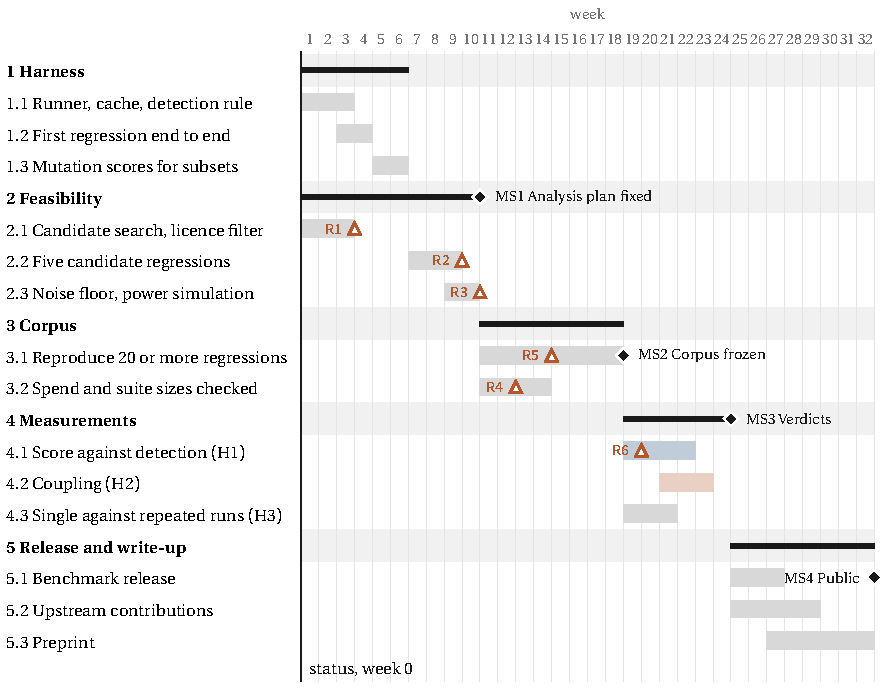
\includegraphics[width=\linewidth]{figures/gantt}
  \caption{\lead{Gantt chart of the project.} Bars are pale where the work is planned and dark where it is done; no work is done yet. Diamonds are milestones and triangles are the risk triggers of \cref{tab:risks}.}
  \label{fig:gantt}
\end{figure}

\section{Risks}

\Cref{tab:risks} gives each risk a trigger, the check that shows whether it has come true, and the week that check falls in.

\begin{table}[tbp]
  \caption{\lead{Risks and fallbacks.} Each trigger is the check that shows whether the risk has come true, with its week, marked R1 to R6 in \cref{fig:gantt}.}
  \label{tab:risks}
  \begin{tabularx}{\linewidth}{l >{\raggedright\arraybackslash}X l l l >{\raggedright\arraybackslash}X >{\raggedright\arraybackslash}X}
    \toprule
    \multicolumn{2}{l}{\head{Risk}} & \head{Threatens} & \head{Likely} & \head{Impact} & \head{Trigger} & \head{Fallback} \\
    \midrule
    \textbf{R1} & too few candidates & \badge{H1} \badge{H2} & \level{medium} & \level{high} & under 34 found, week 3 & search more targets \\
    \band \textbf{R2} & too few regressions reproduce & \badge{H1} \badge{H2} & \level{high} & \level{high} & under 3 of 5, week 9 & more targets; else publish \badge{H3} and corpus \\
    \textbf{R3} & corpus too small for \badge{H1} & \badge{H1} & \level{medium} & \level{high} & half-width over 0.2, week 10 & raise the target; else \badge{H1} as an estimate \\
    \band \textbf{R4} & spend over budget & \badge{H1} \badge{H3} & \level{medium} & \level{medium} & projected over budget, week 12 & lower $k$; drop the costliest target \\
    \textbf{R5} & suites too small to subsample & \badge{H1} & \level{medium} & \level{high} & under 3 targets with 30 or more cases, week 14 & compare whole suites, size confound stated \\
    \band \textbf{R6} & muteval cannot mutate a target & \badge{H1} \badge{H2} & \level{medium} & \level{medium} & adapter fails, week 19 & write the adapter, offer it upstream \\
    \bottomrule
  \end{tabularx}
\end{table}

Each trigger is checked in its week. When one fires, the plan moves to its fallback for the weeks that remain and the Gantt chart is redrawn with the new dates. R2 is the risk the project most depends on, which is why the desk search tests the supply of candidates by week 3 and the feasibility package tests reproduction on five of them before any corpus work begins.

The fallbacks differ in what they cost the conclusions. Widening to more targets under R1 or R2 costs time only. Publishing \badge{H3} and the corpus without the other two keeps a result, the size of the error in single-run verdicts, but gives up the headline question. Comparing whole suites under R5 keeps \badge{H1} but brings back the size confound that can produce the correlation on its own~\cite{Papadakis2018}, so a positive $\tau$ would be reported as an upper bound. Lowering $k$ under R4 widens every interval, so the analysis plan fixed at MS1 states the smallest $k$ at which the interval for \badge{H3} can still fall below 5\%. Reporting \badge{H1} as an estimate under R3 keeps the measurement and its interval but gives no verdict, which is the outcome the power simulation exists to prevent.

% The Gantt chart and the risk table are each half a page; the references start
% on a fresh page so that both are set before them.
\clearpage
\bibliographystyle{apsrev4-2}
\bibliography{refs}

\end{document}
